\documentclass{article}

\usepackage[left=80pt,right=80pt]{geometry}
\usepackage[round]{natbib}
\usepackage[french]{babel}
\usepackage[utf8]{inputenc}
\usepackage[T1]{fontenc}
\usepackage{float}
\usepackage{graphicx}
\usepackage{multicol}
\usepackage{caption}
\usepackage{subcaption}
\usepackage{mathtools}
\usepackage{afterpage}
\usepackage[normalem]{ulem}
\usepackage{listings}
\usepackage{xcolor}
\usepackage{hyperref}
\usepackage{csquotes}
\usepackage{booktabs}
\usepackage{multirow}

% Pour l'ajout de Watermark
% \usepackage[printwatermark]{xwatermark}
% \usepackage{lipsum}
% \newwatermark[allpages,color=gray!20,angle=45,scale=3,xpos=0,ypos=0]{NAME}


% Formattage des hyperliensta
\hypersetup{
    colorlinks=true,
    linkcolor=black,
    filecolor=black,
    urlcolor=black,
    citecolor=black
}
\urlstyle{same}

% Change la mise en page des segments de codes
\definecolor{codegreen}{rgb}{0,0.6,0}
\definecolor{codegray}{rgb}{0.2,0.2,0.2}
\definecolor{codepurple}{rgb}{0.58,0,0.82}
\definecolor{backcolour}{rgb}{0.95,0.95,0.95}
\lstdefinestyle{mystyle}{
    backgroundcolor=\color{backcolour},
    commentstyle=\color{codegreen},
    keywordstyle=\color{magenta},
    numberstyle=\tiny\color{codegray},
    stringstyle=\color{codepurple},
    basicstyle=\ttfamily\footnotesize,
    breakatwhitespace=false,
    breaklines=true,
    captionpos=b,
    keepspaces=true,
    numbers=left,
    numbersep=5pt,
    showspaces=false,
    showstringspaces=false,
    showtabs=false,
    tabsize=4
}
\lstset{style=mystyle}

\renewcommand{\contentsname}{Table des matières}
\renewcommand{\listfigurename}{Table des figures}
\renewcommand{\refname}{Bibliographie}
\renewcommand{\lstlistingname}{Segment de codes}
\renewcommand{\lstlistlistingname}{Table des segments de code}
\newcommand\myhead[2]{%
  \multicolumn{1}{l}{\parbox{#1}{\centering #2}}
}

\bibliographystyle{plainnat}

\setlength\parindent{0pt} % Enleve les indentations dans le document

\title{Laboratoire 2\\
  \large Réseau de neurones profond avec apprentissage par renforcement (DQN)\\
  \normalsize Durée : 3 séances}
\author{Christophe Lamarche}
\date{Mise-à-jour: \today}


\begin{document}
\maketitle

\section{Histoire}

\begin{displayquote}
  \begin{center}
    ``\textbf{Les environnements virtuels et les jeux sont à notre avis la plateforme parfaite pour faire le développement et l'évaluation d'algorithme d'apprentissage machine.}'' \smallbreak
    Demis Hassabis (Co-fondateur et CEO de DeepMind) \citep{AlphaGo-movie}
  \end{center}
\end{displayquote}
\smallbreak

La quête de résoudre un jeu de société a longtemps intéressé les mathématiciens. Le jeu d'échecs a été considéré comme un bon défi pour la résolution, car la quantité de mouvements possibles dans une partie étaient supérieurs aux capacités des ordinateurs de l'époque. \citep{Chess-Ai} L'algorithme \textit{minimax} de John Von Neumann \citep{Von-Neumann} a permis la première résolution du jeu d'échecs pouvant rivaliser avec un joueur moyen au milieu des années 1950.

\bigbreak
La montée en popularité de l'apprentissage machine à l'aide des réseaux de neurones a permis à une collaboration avec l'apprentissage par renforcement. Cette alliance a produit des agents surpassant l'entendement humain. Pensons à \textit{AlphaGo} de \textit{DeepMind} qui a défait en 2016 le champion mondial de Go, Lee Sedol \citep{AlphaGo-movie}. Ou bien, l'équipe d'\textit{OpenAi} ayant réussi à produire un agent pouvant rivaliser avec des professionnels aux jeux vidéo \textit{Dota 2} \citep{OpenAi-Dota} et qui cible présentement le mode collaboratif 5 contre 5 de ce même jeu \citep{OpenAi-Five}.

\subsection{Exposé du problème}
Pour le prochain événement d'un club étudiant, on vous confie le projet de produire un modèle pouvant rivaliser avec des participants au jeu \textit{Breakout} de la plateforme \textit{Atari}.

\bigbreak
Mieux connu sous le nom \textit{Atari Breakout}, ce jeu fut conçu originalement pour les arcades et fut exporté sur la console \textit{Atari 2600}. Le but du jeu est simple : détruire le maximum de briques colorées en renvoyant une balle à l'aide d'une plateforme. Ce jeu fut conçu par Nolan Bushnell, Steve Bristow et Steve Wozniak en 1976.

\begin{figure}[H]
  \centering
  \fbox{
\includegraphics[width=0.35\linewidth]{figures/ataribreakout}}
  \caption{Capture d'écran du jeu Atari Breakout}
  \label{fig:capture}
\end{figure}

% https://www.youtube.com/watch?v=co0SwPWoZh0

\bigbreak
Par chance, ce jeu est disponible dans l'environnement \textit{Gym} d'\textit{OpenAI}. Cet environnement a été conçu pour développer et comparer des algorithmes d'apprentissage par renforcement \citep{OpenAi-Gym}. Cet environnement est conçu spécifiquement pour le langage Python et possède une centaine d'environnements différents accessibles directement avec \textit{Gym} et plusieurs autres via des tierces parties \citep{OpenAi-Gym-Env}. Cette librairie a été intégrée dans le milieu de l'intelligence artificielle par ses multiples références dans des papiers recherches \citep{DQN-Article} et que cette librairie est offert sous la licence \textit{MIT}.

% Gym is a toolkit for developing and comparing reinforcement learning algorithms. It supports teaching agents everything from walking to playing games like Pong or Pinball
% Open source interface to reinforcement learning tasks.
% The gym library provides an easy-to-use suite of reinforcement learning tasks.

\bigbreak
Pour concevoir votre modèle, vous tomber sur le papier ``\href{https://storage.googleapis.com/deepmind-media/dqn/DQNNaturePaper.pdf}{\textit{Human-level control through deep reinforcement learning}}'' \citep{DeepMind-DQN} qui met de l'avant une architecture et un algorithme pour produire un agent qui est capable de rivaliser en termes de performance à des joueurs humains pour les jeux de la plateforme \textit{Atari} telle que le jeu \textit{Breakout}. Selon cette recherche, il vous sera possible de produire un agent tel que demandé par votre client.


\section{Préparation du notebook}
\subsection{Configurer le notebook}

Ce laboratoire nécessite beaucoup de calcul pour l'entraînement du modèle qui nécessite un réseau neuronal convolutif. Pour réduire le temps de traitement, il est intéressant d'utiliser le processeur graphique (GPU) offert avec \textit{Colaboratory}. Pour lier un GPU avec un notebook, il faut premièrement se diriger vers l'option ``Paramètres de notebook'' (\textit{Notebook settings}) sous l'onglet ``Édition'' (\textit{Edit}) figure \ref{fig:setting}.

\begin{figure}[H]
  \centering
  \fbox{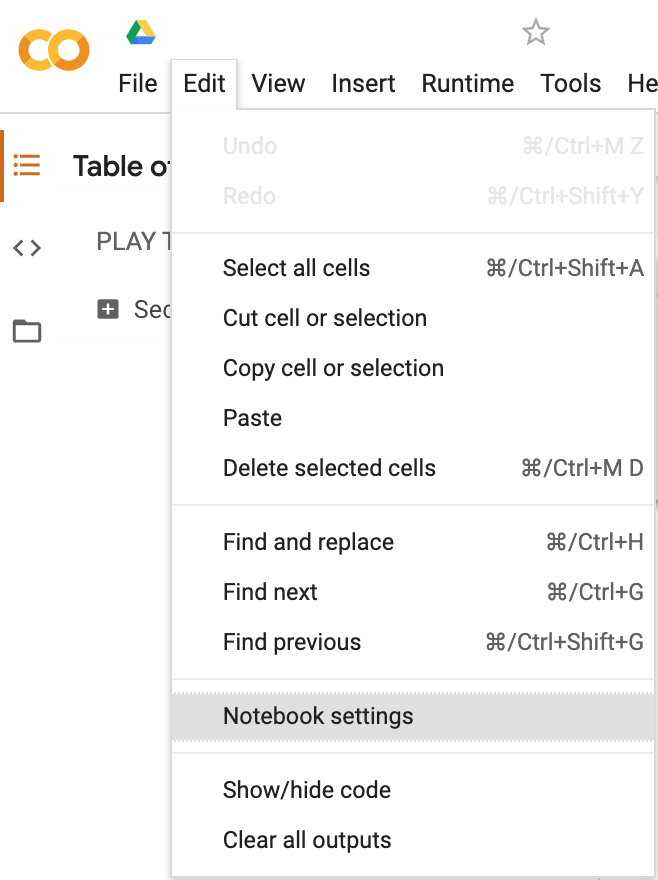
\includegraphics[width=0.5\linewidth]{figures/notebooksettings}}
  \caption{Paramètres du notebook}
  \label{fig:setting}
\end{figure}

Par la suite, sous le menu déroulant, sélectionner GPU tel que dans la figure \ref{fig:selectgpu}. Après avoir sauvegardé les paramètres, connectez le notebook avec une instance de \textit{Colaboratory}.

\begin{figure}[H]
  \centering
  \fbox{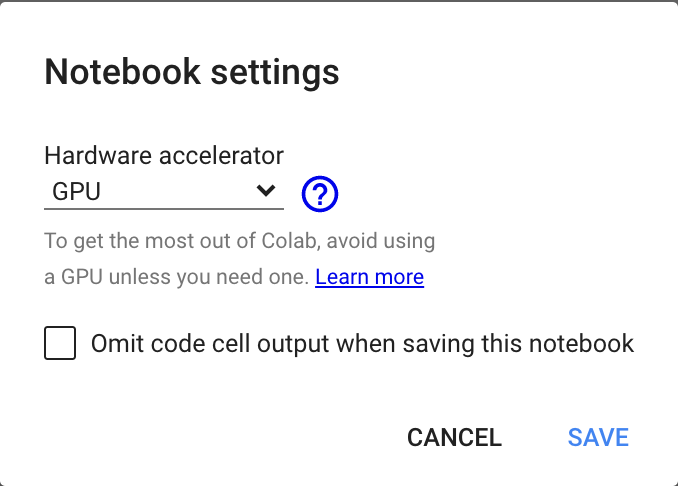
\includegraphics[width=0.5\linewidth]{figures/selectgpu}}
  \caption{Ajout d'un processeur graphique au notebook}
  \label{fig:selectgpu}
\end{figure}

Pour s'assurer que le processeur graphique est bien disponible, utilisez le segment de code \ref{code:gpucheck} dans une cellule de code et faites-en la compilation.

\begin{lstlisting}[language=Python, caption={Valider la présence du GPU}, label={code:gpucheck}]
%tensorflow_version 2.x
import tensorflow as tf
nom_gpu = tf.test.gpu_device_name()
if nom_gpu != '/device:GPU:0':
  raise SystemError('Aucun GPU trouve')
print('GPU trouve : {}'.format(nom_gpu))
\end{lstlisting}

\subsubsection{Librairies à importer}

Pour faire ce laboratoire, quelques librairies devront être importées dans votre projet. Nous voulons utiliser la version 2 de la librairie Tensorflow à l'aide de la commande du segment de code \ref{code:tf2}.

\begin{lstlisting}[language=Python, caption={Sélectionner la version de Tensorflow}, label={code:tf2}]
%tensorflow_version 2.x
\end{lstlisting}

\smallbreak
Si la commande du segment de code \ref{code:tf2} est omise, un avertissement sera affiché lors de l'importation de la librairie ``\textit{Tensorflow}''.

\smallbreak

Les librairies à importer sont :
\begin{itemize}
  \item tensorflow (\textit{tf})
  \item numpy (\textit{np})
  \item skimage.color
  \item cv2
  \item gym
  \item matplotlib.pyplot (\textit{plt})
  \item heapq
  \item json
\end{itemize}

\bigbreak
Tel que dans le laboratoire 1, il est conseillé d'ajouter la commande ``\textbf{\%matplotlib inline}'' au notebook pour simplifier l'affichage des graphiques.
\smallbreak
\textit{Un exemple d'importation de librairies est disponible dans la description du premier laboratoire.}

% Librairies potentielles pour le laboratoire
% % import cv2
% % import numpy as np
% % import random
% % import gym
% % import os
% % import random
% % import tensorflow as tf
% % from tensorflow.keras.initializers import VarianceScaling
% % from tensorflow.keras.layers import (Add, Conv2D, Dense, Flatten, Input, Lambda, Subtract)
% % from tensorflow.keras.models import Model
% % from tensorflow.keras.optimizers import Adam, RMSprop
% % import json
% % import datetime
% % import time
% % import re
% % !python -m pip install array2gif
% % from array2gif import write_gif

% \begin{lstlisting}[language=Python, caption={Importer les librairies}]
% import tensorflow as tf
% from tensorflow.keras import layers
% import numpy as np
% import pandas as pd
% import matplotlib.pyplot as plt
% from scipy import stats
% from sklearn.model_selection import KFold
%
% # Pour l'affichage des figures sans plt.show()
% %matplotlib inline
% \end{lstlisting}

\section{Conception}

Pour simplifier la conception, l'agent est séparé en 2 modules.
\begin{itemize}
  \item Le tampon d'expérience
  \item Deep Q Network (réseau neuronal)
\end{itemize}

\subsection{Constantes du programme (hyperparamêtres)}
Dans la conception d'algorithme d'apprentissage, machine, certains paramètres sont nécessaires d'être définis pour l'entraînement du réseau tel que le taux d'apprentissage, l'architecture du modèle et la taille du \textit{minibatch} utilisée pour l'apprentissage.

\bigbreak
Pour ce laboratoire, les constantes suivantes doivent être définies :
\begin{itemize}
  \item À trouver dans la documentation
  \begin{itemize}
    \item Quantité de départ pour le tampon d'expérience (\textit{replay start size})
    \item Taille du tampon d'expérience (\textit{replay memory size})
    \item Taille du minibatch (\textit{minibatch size})
    \item Historique des états (\textit{agent history length})
    \item Fréquence de mise à jour du réseau cible (\textit{target network update frequency})
    \item Facteur de réduction (\textit{discount factor})
    \item Quantité de répétition des actions (\textit{action repeat})
    \item Valeur initiale de l’epsilon pour $\epsilon-greedy$ (\textit{initial exploration})
    \item Valeur finale de l’epsilon pour $\epsilon-greedy$ (\textit{final exploration})
    \item Index de la dernière image d'exploration $\epsilon-greedy$ (\textit{final exploration frame})
    \item Nom de l'environnement (\textit{sous la forme ``NomDuJeu-vX''})
  \end{itemize}
  \item Offert par l'auteur
  \begin{itemize}
    \item Taille de l'image préprocessée \textbf{(84, 84)} pixels
    \item Nombre d'épisodes à effectuer \textbf{(3500)}
  \end{itemize}
\end{itemize}

\bigbreak
Certains de ces hyperparamêtres sont facilement disponibles dans les documentations en lien avec le projet. À l'aide des liens suivants, déterminez la valeur des hyperparamêtres.
\begin{itemize}
  \item \href{https://storage.googleapis.com/deepmind-media/dqn/DQNNaturePaper.pdf}{https://storage.googleapis.com/deepmind-media/dqn/DQNNaturePaper.pdf}
  \item \href{https://gym.openai.com/}{https://gym.openai.com/}
\end{itemize}


\subsection{Intégration de l'environnement}
L'environnement gym d'OpenAI est conçu afin que tous les environnements possèdent la même interface de programmation (\textbf{API}). Avec le temps, cette interface est devenue l'interface par défaut qu'un environnement doit respecter pour être accueilli par la communauté d'apprentissage par renforcement.

\subsubsection{Produire un environnement}
À l'aide de la libraire ``gym'', il faut utiliser la fonction ``make'' du module avec le nom de l'environnement comme argument (segment de code \ref{code:env}).

\bigbreak
\begin{lstlisting}[language=Python, caption={Création de l'environnement}, label={code:env}]
env = gym.make(NOM_DU_JEU)
\end{lstlisting}

\subsubsection{Extraire les actions utilisées par l'environnement}
Comme tous jeux, les actions entre les différents environnements diffèrent. Une des manières pour extraire les définitions des commandes sur un environnement ``gym'' est d'utiliser la suite de méthodes du segment de code \ref{code:actions}.

\bigbreak
\begin{lstlisting}[language=Python, caption={Extraire les actions utilisées par l'environnement}, label={code:actions}]
NOMBRE_ACTION = len(env.unwrapped.get_action_meanings())
\end{lstlisting}

\subsubsection{Interactions avec l'environnement}

Pour obtenir l'image de l'environnement, deux méthodes sont disponibles. La première est d'effectuer une action à l'aide de la méthode \textbf{step}. Cette méthode retourne un ``\textit{tuple}'' de quatre arguments : l'image résultante, la récompense, la valeur du drapeau de fin et un dictionnaire d'information dont le nombre de vies restant. La deuxième méthode est à l'aide de la méthode \textbf{render} qui fait un rendu sans le besoin d'action. Comparativement à \textbf{step}, \textbf{render} retourne seulement la dernière image produite par l'environnement. Il est à noter que la méthode \textbf{render} est possible qu'après avoir fait une action dans un nouvel environnement.

\bigbreak
\begin{lstlisting}[language=Python, caption={Initilisation Gym pour Atari Breakout v0}, label={code:initgym}]
# Importer l'environnement Breakout-v0
env = gym.make('Nom de l'environnement')
# Repartir l'environnement a l'etat initial
env.reset()

# Liste des definitions des actions
env.unwrapped.get_action_meanings()

# Rendu de l'environnement
env.render(mode='rgb_array')

# Faire une action dans l'environnement
env.step(action, render_mode='rgb_array')
\end{lstlisting}


\subsection{Tampon d'expérience}
Le tampon d'expérience est l'un des deux modules devant être conçus pour produire l'algorithme DQN \citep{DQN-Article}. Pour bien concevoir ce module, nous allons mettre sur pied une classe. Cette classe aura comme but de mettre en mémoire des expériences de l'environnement.

\subsubsection{Expérience}
Le papier mettant en lumière l'algorithme du \textit{DQN} fait aussi l'utilisation du principe de tampon d'expérience (\textit{replay buffer}). L'apprentissage à l'aide d'expérience consécutive pour un agent \textit{DQN} est inefficace \citep{DQN-Article}. Le tampon d'expérience fera la sélection d'expérience de manière aléatoire.

\medbreak
$$e_{t} = (s_{t},a_{t},r_{t},s_{t+1})$$

\bigbreak
Une expérience est définie comme la composition de l'image d'origine ($s_{t}$), l'action choisie par rapport à cette image ($a_{t}$), la récompense résultante ($r_{t}$) et l'image produite ($s_{t+1}$) \citep{DQN-Article}.

\bigbreak
Ces composantes sont offertes par l'environnement ``gym'' lorsqu'une action est effectuée avec la méthode ``step''.

\subsubsection{Création de la classe ``\textit{TamponExperience}''}
Python étant un langage orienté objet, les modules seront conçus sous la forme d'un objet. Avec Python, un objet se réfère lui-même à l'aide du mot ``\textit{self}''. De plus, plusieurs méthodes dites \textit{spéciales} sont réservées pour décrire des interactions souvent utilisées. Par exemple, la méthode ``\textbf{\_\_init\_\_}'' est appelée lors de la création d'un nouvel objet d'une classe pour son initialisation \citep{Python-Method}. Cette méthode \textit{spéciale} est celle-là plus couramment modifiée lors de l'écriture d'une classe.

\bigbreak
Similaire à ``\textbf{def}'' pour la création d'une fonction, le terme ``\textbf{class}'' sert à indiquer la conception d'une nouvelle classe. Le segment de code \ref{code:classe} offre un exemple pour le début de la création d'une classe.
\bigbreak
% TODO : Vérifier que la phrase ci-dessous reste vrai à la fin du laboratoire.
Pour ce laboratoire, le champ ``\textit{héritage}'' sera laissé vide.

\begin{lstlisting}[language=Python, caption={Création d'une classe en Python}, label={code:classe}]
class Nom_de_la_classe(heritage):
  [...]
\end{lstlisting}

\subsection{Fonction d'initialisation}
À l'intérieur d'une classe, il est nécessaire de définir une méthode faisant l'initialisant d'un objet. Cette méthode est appelée au premier appel de la classe. Le segment de code \ref{code:initrectangle} montre un exemple d'initialisation pour une classe fictive \textbf{Rectangle}.

\bigbreak
\begin{lstlisting}[language=Python, caption={Initilisation d'une classe d'un rectangle}, label={code:initrectangle}]
class Rectangle():
  def __init__(self, largeur, hauteur):
    """
    __INIT__

    Initialisation d'un objet Rectangle

    @Arguments :
      largeur {float} : largeur du rectangle [en unite de distance]
      hauteur {float} : hauteur du rectangle [en unite de distance]

    @Return :
      {Rectangle} : l'objet Rectangle ayant appeler la fonction.

    ** Note : il n'est pas necessaire de mettre 'return self' pour __init__
    """
    self.largeur = largeur
    self.hauteur = hauteur
    self.perimetre = 2 * (self.largeur + self.hauteur)
    self.aire = self.largeur * self.hauteur
    return self
\end{lstlisting}

En Python, la mention \textbf{self} est un pointeur correspondant à l'objet même. \textbf{Self} est similaire au pointeur \textbf{this} dans d'autres language comme \textbf{c++} et \textbf{JavaScript}. En appelant une composante de \textbf{self}, il est possible de la définir (segment de code \ref{code:initrectangle}) et de l'utiliser (segment de code \ref{code:userectangle}).

\bigbreak
\begin{lstlisting}[language=Python, caption={Appel de la classe Rectange}, label={code:userectangle}]
r = Rectangle(5,6)
print('Aire du rectangle:',r.aire) # >> Aire du rectangle: 30
\end{lstlisting}

\subsection{Initialisation du tampon}
Pour le tampon d'expérience, nous utilisons quatre tampons circulaires qui contiendront les valeurs d'actions, les récompenses, les images traités et les drapeaux de fins aux instant \textbf{t}.

\bigbreak
Les tampons circulaires sont de la taille maximale du tampon d'expérience. L'allocation de ces tampons sont fait à l'aide de la fonction ``numpy.empty''. De cette manière, nous contournons les problématiques d'épuisement de mémoire pouvant être produit par le \textit{collecteur de vidange (Garbage collector)}.

\bigbreak
\begin{lstlisting}[language=Python, caption={Allocation du tampon contenant les images}, label={code:alloc}]
self.images = np.empty((taille_max_tampon, hauteur_image_traitee, largeur_image_traitee), dtype=np.uint8)
\end{lstlisting}

\bigbreak
Le but du tampon est de contenir l'information, alors il est nécessaire d'utiliser le type pouvant correspondant aux données sans utiliser de l'espace mémoire superflu.

\begin{figure}[H]
  \centering
  \fbox{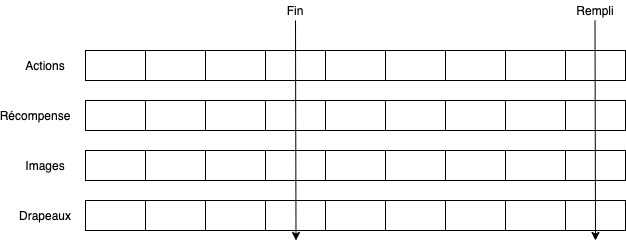
\includegraphics[width=0.5\linewidth]{figures/tampon}}
  \caption{Schématisation d'un tampon circulaire}
  \label{fig:tampon}
\end{figure}

\bigbreak
\textbf{Faites l'allocation des trois autres tampons}
\bigbreak

Pour interagir avec les tampons, nous devons utiliser trois variables pour définir l'état de ceux-ci. La première variable contient la taille maximale du tampon (\textit{taille}). La deuxième variable indique combien de valeur est contenu dans le tampon à l'instant \textbf{t} (\textit{compteur}) et d'une variable utilisée comme pointeur pour donner la position de la prochaine valeur à ajouter.

\bigbreak
Afin de réduire l'utilisation de mémoire par le tampon d'expérience, il est intéressant de faire l'allocation d'espace mémoire pour la création des \textit{minibatchs}. Pour cela, nous allons allouer l'espace pour trois matrices. Deux allant contenir des états qui seront traités par les réseaux neuronaux (segment de code \ref{code:allocetat}) et une matrice contenant les indices utilisés pour la conception des états.

\bigbreak
\begin{lstlisting}[language=Python, caption={Allocation de la matrice pour contenir les états}, label={code:allocetat}]
self.etat = np.empty((taille_minibatch, historique, hauteur_image_traitee, largeur_image_traitee), dtype=np.uint8)
\end{lstlisting}


\subsubsection{Traitement de l'image}
La première modification qui influencera directement l'agent est le traitement de l'image pour réduire la complexité de l'image produite par l'environnement.

\bigbreak
Selon l'article original faisant mention de l'architecture ``\textit{Deep Q-Network}'' \citep{DQN-Article}, lors de leur conception avec les jeux de la plateforme \textit{Atari 2600}, les images reçues par l'environnement sont réduites à une dimension de 84 pixels par 84 pixels en ton de gris avant d'être envoyées au modèle. Il est important que l'image traitée soit carrée pour être compatible avec les couches de convolution 2D au début du modèle.

\begin{center}
  \begin{tabular}{| l | c | c |}
    \hline
    Propriétés  & Originale           & Traitée \\
    \hline
    Taille      & 210 x 160 pixels    & 84 x 84 pixels \\
    Couleur     & RGB (128 couleurs)  & Ton de gris (0,255)\\
    Contenu     & Totalité de l'écran & Section de jeu \\
    \hline
  \end{tabular}
\end{center}

\begin{figure}[H]
\centering
\begin{minipage}{.5\textwidth}
  \centering
  \fbox{
\includegraphics[width=0.75\linewidth]{figures/ataribreakout}}
  \captionof{figure}{Image tirée de l'environnement \textit{Gym}}
  \label{fig:breakout_original}
\end{minipage}%
\begin{minipage}{.5\textwidth}
  \centering
  \fbox{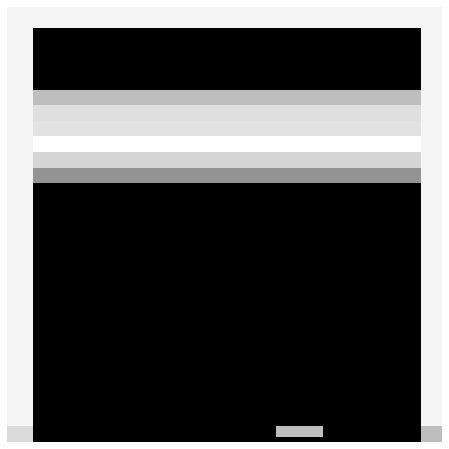
\includegraphics[width=0.75\linewidth]{figures/atariprocessed}}
  \captionof{figure}{Image traité pour le modèle.}
  \label{fig:breakout_preprocessed}
\end{minipage}
\end{figure}

\bigbreak
Les fonctions qui sont à votre disposition pour faire le traitement sont :
\begin{itemize}
  \item tensorflow.image.rgb\_to\_grayscale
  \item tensorflow.image.crop\_to\_bounding\_box
  \item tensorflow.image.resize (avec la méthode \textbf{tensorflow.image.ResizeMethod.NEAREST})
  \item la méthode de reshape de la matrice \textit{numpy}
\end{itemize}

\bigbreak
Pour ajouter une méthode dans une classe, il faut simplement ajouter une fonction à l'intérieur de la classe avec l'indentation correspondante .

\bigbreak
\begin{lstlisting}[language=Python, caption={Définition d'une méthode statique}, label={code:method}]
class Rectangle()
  def __init__(self, largeur, hauteur):
    ...

  def calculer_aire(self):
    """
    CALCULER_AIRE

    Calculer l'aire d'un rectangle a l'aide d'un objet Rectangle.

    @Arguments :
      self {Rectangle} : Objet faisant l'appel de la methode

    @Return :
      {float} : Aire du rectangle correspondant
    """
    return self.largeur * self.hauteur
\end{lstlisting}

\bigbreak
Lorsqu'une méthode offre des fonctionnalités similaires à un objet, mais ne nécessite pas l'utilisation d'attribut d'un objet, il est possible de définir une méthode statique à l'intérieur d'une classe. Ceci offre la possibilité d'appeler la fonction sans définir un objet auparavant. Pour définir une méthode statique, il suffit d'ajouter le décorateur ``@staticmethod'' avant la méthode.

\bigbreak
\begin{lstlisting}[language=Python, caption={Définition d'une méthode statique}, label={code:static}]
class Rectangle()
  def __init__(self, largeur, hauteur):
    ...

  @staticmethod
  def calculer_aire(largeur, hauteur):
    """
    CALCULER_AIRE

    Calculer l'aire d'un rectangle a l'aide de la largeur et de la hauteur.

    @Arguments :
      largeur {float} : Largeur du rectangle
      hauteur {float} : hauteur du rectangle

    @Return :
      {float} : Aire du rectangle correspondant
    """
    return largeur * hauteur
\end{lstlisting}

\textbf{Un exemple d'image du jeu est offert lors de la réinitialisation de l'environnement ``gym'' (env.reset())}

\subsubsection{Ajout d'une expérience dans le tampon}
Pour ajouter une expérience à l'intérieur du tampon, il suffit de prendre les composantes d'une expérience (image, récompense, action, drapeau de fin) et de les insérer dans leur tampon respectif où le pointeur de donnée indique. Par la suite, les variables de contrôle du tampon sont mises à jour. Le compteur est incrémenté d'un incrément jusqu'à ce qu'il soit identique à la taille du tampon. Pour sa part, le pointeur est incrémenté d'un incrément et est restreint à l'intérieur de la taille du tampon (utiliser l'opération modulo \%).

\subsubsection{Déterminer les indices pour la création d'un état}
La classe du tampon d'expérience est utilisée pour la manipulation des données. Il est donc nécessaire de définir une méthode pour extraire une suite d'index pour concevoir des états pour l'apprentissage du modèle. Pour ce faire, nous devons définir une boucle ayant comme but de produire une quantité précise d'indices aléatoires respectant des conditions précises.

\bigbreak
Les conditions à respecter sont :
\begin{itemize}
  \item Si l'index est plus grand que le pointeur, alors l'indice doit avoir au moins une différence minimum de la taille de l'historique avec un incrément de 1.
  \item Si le compteur n'est pas équivalent à la taille maximale du tampon, l'index doit être supérieur à l'historique avec un incrément de 1
  \item Il ne doit pas avoir de drapeaux de fin entre l'index choisie et les indexes contenus à l'intérieur de l'historique
\end{itemize}

\bigbreak
La dernière condition s'assure que les valeurs qui seront à l'intérieur de l'état sont du même épisode. Lorsqu'un indice respecte toutes les conditions, ajouter cette valeur à l'intérieur de la matrice devant contenir les indices des états.

\bigbreak
\textit{Le but de la tâche est de respecter la distribution uniforme d'une sélection aléatoire. Alors, il n'est pas nécessaire de s'assurer si un indice a déjà été sélectionné.}

\subsubsection{Création d'un état}
Dans le cas de ce laboratoire, un état correspond à l'agrégation d'observation (image). Pour produire une sous-matrice, il est possible d'utiliser une indexation bornée. L'indexation bornée est faite en sorte que la borne inférieure est incluse et celle supérieure est exclue.

\bigbreak
\begin{lstlisting}[language=Python, caption={Indexation bornée}, label={code:index}]
a = [[1,2,3],[4,5,6],[7,8,9]]
a[0:2] # >> [[1,2,3],[4,5,6]]
\end{lstlisting}
\bigbreak

À l'aide de cette information, créer une méthode pouvant extraire les images d'un index précis et son historique.
\bigbreak

\begin{figure}[H]
  \centering
  \fbox{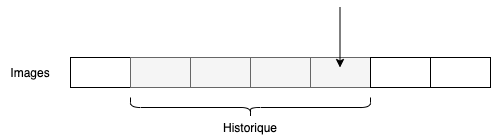
\includegraphics[width=0.5\linewidth]{figures/indexation}}
  \caption{Extraction d'un état}
  \label{fig:index}
\end{figure}

\subsubsection{Création d'un minibatch}
Le minibatch est le regroupement de plusieurs entrées afin que le modèle fasse leur traitement simultanément. Cette technique aide à réduire la quantité de bruit dans les gradients pouvant être produit par une donnée disparate.

\bigbreak
\begin{lstlisting}[language=Python, caption={Création d'un minibatch}, label={code:minibatch}]
def creer_minibatch(self):
  trouver_indices_valide(nombre_donnees_par_minibatch)

  # Une boucle enumerate sert a indique la position de la valeur sortie simultanement
  for i, index in enumerate(self.indices) :
    etats[i] = creer_etat(index-1)
    etats_suivant[i] = creer_etat(index)

  return etats, actions[self.indices], recompenses[self.indices], etats_suivant, drapeaux[self.indices]
\end{lstlisting}

L'état offert par le segment de code \ref{code:minibatch} a toutefois la problématique qu'une couche peut avoir de la difficulté à traiter l'information temporelle de l'état, car il n'est pas situé à la dernière dimension de la matrice. Pour corriger cela, il suffit d'utiliser la fonction ``numpy.transpose'' avec l'argument ``axis=(0,2,3,1)''. De cette manière, nous prenons la deuxième dimension de la matrice et la transporte à la dernière dimension.

\subsubsection{Produire un nouvel état à partir de l'état précédent}
Cette dernière fonction du tampon d'expérience a comme but simple de prendre un état et d'y intégrer une nouvelle image traitée en retirant l'image la plus ancienne de l'état.

\subsection{Modèle}
Avec la gestion d'expérience compléter, il est maintenant nécessaire de construire le réseau de neurones. Le modèle utilisé dans l'algorithme \textit{DQN} est divisible en quatre parties.

\bigbreak
La première section du modèle est l'entrée du modèle. Cette couche définit l'entrée afin que \textit{tensorflow} puisse définir l'espace nécessaire pour la conception du réseau neuronal lors de la compilation (\textit{tensorflow.keras.Input}).

\bigbreak
La deuxième section est de formater l'entrée. Dans le tampon d'expérience, nous gardons en mémoire l'intensité des pixels sous le format ``uint8''. Cette représentation a peu de valeur pour le réseau. Pour remédier à la situation, nous allons formater les pixels afin que les valeurs soit entre 0 et 1. Pour ce faire, nous utilisons la couche \textbf{tensorflow.keras.Lambda} pour diviser par 255.

\bigbreak
La couche \textbf{Lambda} traite les données en entrées par une fonction personnalisée. Afin de faciliter l'écriture de cette couche, nous utilisons la création de fonctions à l'aide de la définition simplifiée \textit{lambda}. \textit{Lambda} retourne le résultat du traitement à droite de ``:'' (segment de code \ref{code:lambda}).

\textit{D'avantage d'information est disponible sous la documentation de la couche : \href{https://www.tensorflow.org/api\_docs/python/tf/keras/layers/Lambda}{https://www.tensorflow.org/api\_docs/python/tf/keras/layers/Lambda}}.

\bigbreak
\begin{lstlisting}[language=Python, caption={Utilisation de la définition par lambda}, label={code:lambda}]
nom_fonction = lambda entree: traitement(entree)
\end{lstlisting}

\bigbreak
La troisième section est un réseau convolutif pour l'analyse de l'image. Les réseaux convolutifs sont souvent utilisés dans la catégorisation d'image (AlexNet, ResNet, ...).

Alors, cette section a comme but de déterminer par itérations les caractéristiques importantes du jeu par l'entremise de la sortie de l'environnement. Le réseau convolutif est constitué de 3 couches. Dans la librairie \textit{tensorflow}, il existe trois types de couches de convolution. Dans le laboratoire, nous nous intéressons à la couche de convolution à deux dimensions (\textbf{Conv2D}).

\bigbreak
  \begin{table}[H]
  \centering
  \begin{tabular}{|@{}ccccc@{}|}
    \hline
    Index &
    \myhead{2.3cm}{Profondeur de \\ sortie (\textit{filters})} &
    \myhead{2.3cm}{Dimension \\ de noyau} &
    \myhead{2.3cm}{Déplacement \\ (\textit{stride})} &
    Fonction d'activation \\
    \hline
    1 & 32 & $8\times8$ & 4 & relu \\
    2 & 64 & $4\times4$ & 2 & relu \\
    3 & 64 & $3\times3$ & 1 & relu \\
    \hline
  \end{tabular}
  \caption{Description des couches de convolution}
  \label{table:conv2d}
\end{table}
\bigbreak

Afin de faire le lien entre une entrée bidimensionnelle et une couche totalement connectée, il est nécessaire d'ajouter une couche d'aplatissement (\textbf{Flatten}).

\bigbreak
La dernière couche du modèle est un perceptron. Cette couche complètement connectée fait le lien entre l'observation des couches de convolution et les commandes de l'environnement. Le perceptron est constitué de 512 neurones terminés par la fonction d'activation \textit{relu} suivie de 4 neurones représentant les actions de l'environnement du jeu \textit{Atari Breakout}.

\begin{figure}[H]
  \centering
  \fbox{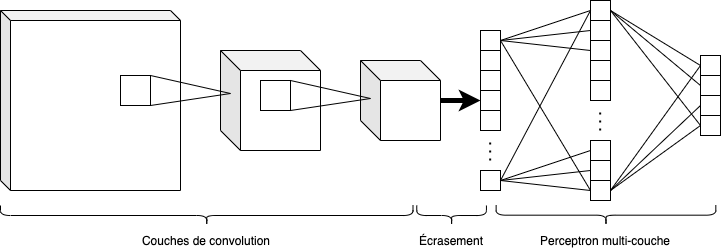
\includegraphics[width=0.9\linewidth]{figures/model}}
  \caption{Schéma du modèle}
  \label{fig:modele}
\end{figure}

Dans ce laboratoire, le modèle utilise l'optimisateur Adams pour la mise à jour des poids et de la fonction de pertes Huber.
\bigbreak
\begin{lstlisting}[language=Python, caption={Compilation du modèle}, label={code:compile}]
model.compile(optimizer=tf.keras.optimizers.Adam(1e-5), loss=tf.keras.losses.Huber())
\end{lstlisting}

\subsubsection{Initialisation du modèle}
La conception du modèle devra être faite à l'intérieur d'une fonction afin de pouvoir répliquer le modèle aisément.

\bigbreak
La fonction d'initialisation possède deux variables dans sa création. La première variable est la taille de l'image en entrée. La taille de l'image étant déjà définie dans le papier de recherche du DQN. Toutefois, il est intéressant d'offrir la possibilité de modifier ce paramètre dans le futur. La deuxième variable est le nombre d'actions possibles pour l'environnement. De cette manière, il sera possible de réutiliser l'algorithme sur différents jeux de l'environnement \textit{Gym d'OpenAI}.


% model = Model(model_input, q_vals)
% model.compile(Adam(learning_rate), loss=tf.keras.losses.Huber())

\bigbreak
Avec les techniques utilisées dans le premier laboratoire, faites la création du réseau de neurones.

\subsubsection{Entraînement du réseau}
La méthode d'entraînement diverge de celui du premier laboratoire en utilisant un aspect davantage manuel au procédé. Dans ce laboratoire, nous utilisons la fonction de perte de l'algorithme \textbf{DQN} pour mettre à jour les poids.

$$L(\theta) = E_{s,a,r,s'}[(r + \gamma max_{a'}\hat{Q}_{\theta'}(s',a')-Q_{\theta}(s,a))^{2}]$$

\bigbreak
Cette équation possède trois segments distinctifs. Le premier segment est $G(r,s',a') = r + \gamma max_{a'}\hat{Q}_{\theta'}(s',a')$ qui correspond à la valeur Q voulue pour le réseau de neurones. Cette équation est la somme entre la valeur Q du réseau cible et de la récompense de l'action obtenue. Le deuxième segment est $Q_{\theta}(s,a)$ qui correspond à la valeur Q obtenue par le réseau de neurones interagissant avec l'environnement. Finalement, nous calculons la distance euclidienne (L2) entre les deux valeurs. Le préfix $E_{s,a,r,s'}$ indique que le résultat obtenu correspond à la valeur attendue.

\bigbreak
Dans le cas du laboratoire, nous utilisons l'outil \textit{GradientTape} de \textit{Tensorflow} pour capter le gradient du réseau de neurones. De cette manière, il sera possible d'analyser précisément la fonction de perte de l'algorithme DQN.

\bigbreak
Dans le Segment de code \ref{code:gradienttape}, nous utilisons la représentation ``\textit{one-hot}'' pour cibler la valeur Q obtenus par le réseau de neurones. La représentation ``\textit{one-hot}'' correspond à une matrice unidimensionnelle dont toutes les valeurs sont forcées à zéro sauf l'indice voulu qui est forcé à un.

\bigbreak
Par exemple, la représentation ``\textit{one-hot}'' de la valeur 3.5 avec une matrice avec une profondeur de 5 correspond à la matrice $\begin{bmatrix}0 & 0 & 0 & 1 & 0\end{bmatrix}$.

\bigbreak
Pour faciliter la conception de l'entraînement du modèle, nous utilisons l'outil ``GradientTape'' offert par Tensorflow qui fait automatique le calcul des gradients pour la mise à jour des poids. De plus, nous remplaçons la fonction de pertes ``MSE'' par la fonction \textbf{Huber} qui offre une forme similaire, mais dont la pente devient constante lorsque l'erreur est trop grande. Cela aide à réduire la possibilité de divergence du modèle.

\bigbreak
\begin{lstlisting}[language=Python, caption={Utilisation de GradientTape}, label={code:gradienttape}]
with tf.GradientTape() as tape :
  # Informe quoi gradientTape doit analyser
  tape.watch(self.model.trainable_variables)

  Qs = model.predict(states)
  Q = tf.reduce_sum(Qs * tf.one_hot(actions, self.nbr_action),axis=-1)

  # Calcul des pertes
  pertes = tf.reduce_mean(self.model.loss(G, Q))

gradients = tape.gradient(pertes, self.model.trainable_variables)
self.model.optimizer.apply_gradients(zip(gradients, self.model.trainable_variables))
\end{lstlisting}

\bigbreak
Avec l'information offerte par le Segment de code \ref{code:gradienttape}, nous pouvons en déduire que la fonction d'entrainement nécessite comme arguments l'expérience, la valeur Q du réseau de comparaison et d'un accès au réseau de neurones du modèle.

\subsubsection{Transfert des valeurs des poids entre deux modèles}
Les méthodes faisant la lecture des poids d'un modèle \textit{Tensorflow} sont \textbf{get\_weights} et \textbf{set\_weights}. À partir de ces méthodes, faites la conception de la méthode pouvant transférer les poids du modèle principal vers le modèle comparatif.

\subsubsection{Choix d'une action}
L'algorithme du DQN \citep{DQN-Article} utilise $\epsilon-greedy$ pour l'exploration et l'évaluation du modèle.

\bigbreak
\begin{itemize}
  \item Si une valeur aléatoire entre 0 et 1 est inférieure à la valeur epsilon ($\epsilon$)
  \begin{itemize}
    \item Retourne une action aléatoire
  \end{itemize}
  \item Sinon
  \begin{itemize}
    \item Retourne l'argmax du résultat du modèle pour l'état.
  \end{itemize}
\end{itemize}

\subsection{Jouer un épisode}
Les étapes pour jouer un épisode avec l'algorithme DQN \citep{DQN-Article}.
\bigbreak
\begin{enumerate}
  \item réinitialiser l'environnement
  \item Aggréger l'image initiale pour produire un état
  \item Tant que le drapeau de fin n'est pas levé
  \begin{enumerate}
    \item si un nombre ``t'' d'actions a été vu, transférer les poids du modèle principal vers le modèle de comparaison
    \item prendre une action avec $\epsilon-greedy$
    \item effectuer l'action sur l'environnement
    \item ajouter les résultats de l'action dans le tampon
    \item incrémenter le nombre ``t'' d'actions vues
    \item réduire la valeur d'epsilon ($\epsilon$)
    \item faire l'apprentissage du modèle en utilisant un minibatch du tampon
    \item l'état est mis à jour avec la nouvelle image traitée obtenue à l'aide de l'action précédente.
  \end{enumerate}
\end{enumerate}

\bigbreak
Il est recommandé de faire la sommation des récompenses offerte par l'environnement pour déterminer les performances du modèle.

\bigbreak
Avec cette information, produisez une fonction implémentant le jeu d'un épisode.

\bigbreak
Pour faciliter votre conception, il est conseillé que cette fonction reçoit en argument :
\bigbreak
\begin{itemize}
  \item l'environnement
  \item la valeur ``t''
  \item le tampon d'expérience
  \item le modèle principal
  \item le modèle comparatif
  \item la valeur epsilon ($\epsilon$)
\end{itemize}

\bigbreak
En fin de conserver les modifications avec certains de ces arguments, il est nécessaire de renvoyer les valeurs :
\begin{itemize}
  \item la valeur ``t'' actualisée
  \item la valeur epsilon ($\epsilon$)
  \item le résultat de l'épisode
\end{itemize}

\subsection{Algorithme DQN}
La dernière étape à la conception du laboratoire est de joindre tous les modules pour produire l'algorithme du DQN \citep{DQN-Article}.

\bigbreak
\begin{enumerate}
  \item Initilisation du tampon d'expérience afin d'attendre la borne inférieure en effectuant que des actions aléatoires.
  \item Initilisation du modèle principal et du modèle comparatif.
  \item Copier les poids du modèle principal vers le modèle comparatif.
  \item Pour un nombre M d'épisodes
  \begin{enumerate}
    \item jouer une partie
  \end{enumerate}
\end{enumerate}

\section{À mettre dans le rapport} % Document à remettre
Avec le rapport, il faut remettre le notebook (`.ipynb') et le dossier ``modeles''
\medbreak

Pour télécharger le fichier du notebook, cliquez l'option ``Télécharger .ipynb'' (\textit{``Download .ipynb''}) sous l'onglet fichier.

\begin{figure}[H]
  \centering
  \fbox{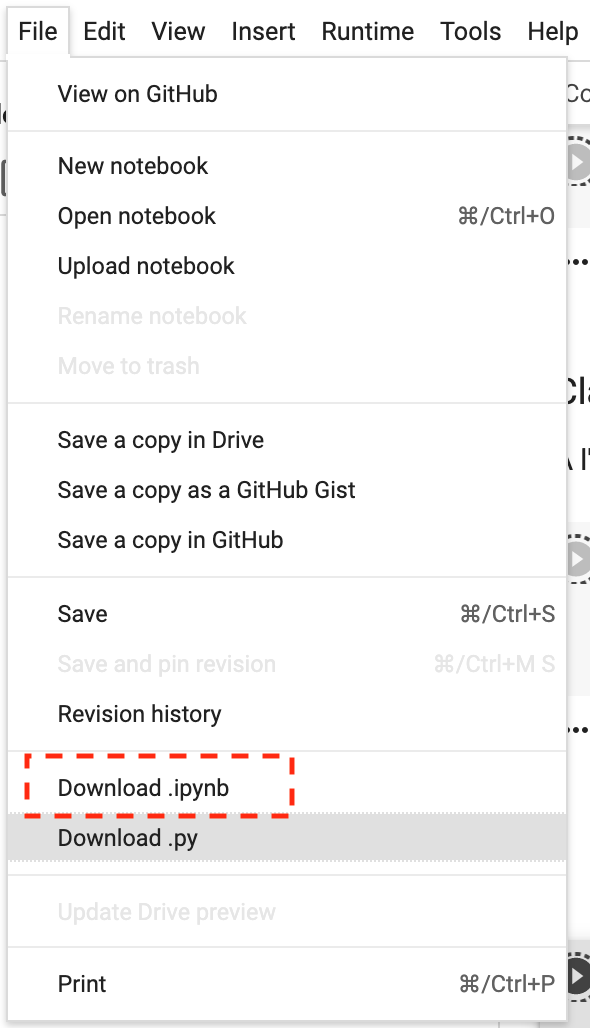
\includegraphics[height=0.75\linewidth]{figures/downloadipynb}}
  \caption{Télécharger le notebook}
  \label{fig:downloadipynb}
\end{figure}
\medbreak
Afin de télécharger le dossier ``modeles'', il faut le compresser auparavant. Pour se faire, ouvrer une nouvelle cellule de code et insérer la commande ci-dessous.

\begin{lstlisting}[language=Python, caption={Compresser un fichier sur une session}, label={code:zip}]
!zip -r modeles.zip ./modeles
\end{lstlisting}
\smallbreak
\textit{Faites attention au point d'exclamation [!] au début de la commande}

\medbreak
Par la suite, il est possible de télécharger en se dirigeant sur l'icône de fichier dans la barre de gauche du notebook tel que représenté dans la figure \ref{fig:downloadzip}.
\begin{figure}[H]
  \centering
  \fbox{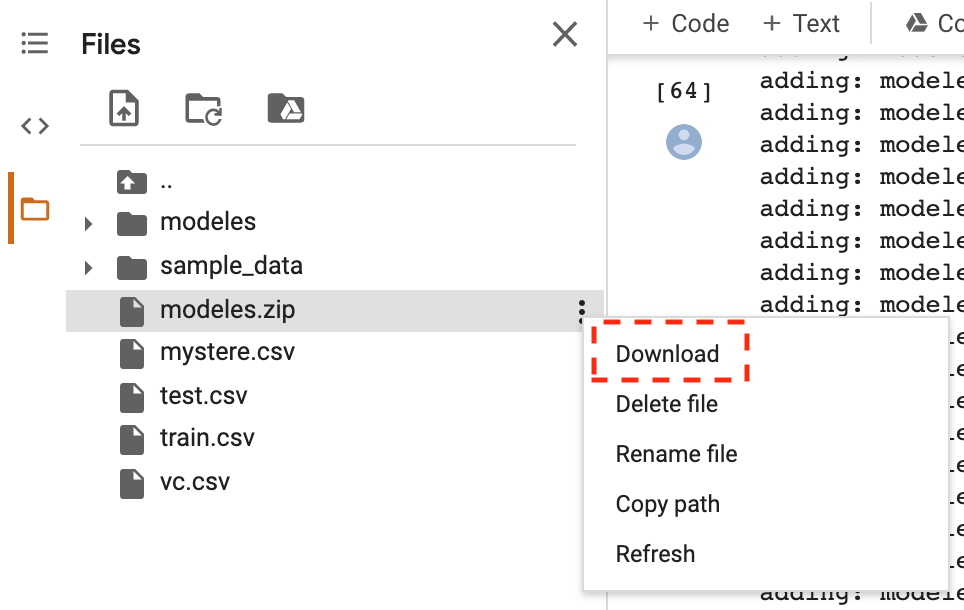
\includegraphics[width=0.75\linewidth]{figures/downloadzip}}
  \caption{Télécharger le dossier compressé}
  \label{fig:downloadzip}
\end{figure}

\begin{table}[H]
  \caption{Contenu du rapport}
  \label{tab:remettre}
  \centering
  \begin{tabular}{|l|l|l|c|}
    \hline
    Section & Taille minimum & Pondération \\
    \hline
    Introduction & 3 lignes & 5\%\\
    Théorie & 5 lignes & 20\%\\
    Résultats & 5 lignes & 40\%\\
    Conclusion & 5 lignes & 35\%\\
    \hline
  \end{tabular}
\end{table}

\subsection{Description des sections}
\subsubsection{Introduction}
Dans l'introduction, il faut décrire le but du laboratoire et de résumer la procédure du laboratoire.

\subsubsection{Théorie}
Dans la section théorique, il est nécessaire d'expliquer les théories et les concepts qui sont mis de l'avant par le laboratoire.

\subsection{Résultats}
La section des résultats doit inclure les graphiques, les tableaux obtenus durant le laboratoire. Il est nécessaire d'inclure une figure décrivant l'entrainement pour chaque modèle. De plus, il est nécessaire d'expliquer le résultat observé à l'intérieur de la figure.

\subsubsection{Conclusion}
Finalement, la conclusion doit contenir un simple retour sur le but, une évaluation des résultats et une ouverture sur l'amélioration du laboratoire.

%
% \begin{figure}[H]
%   \centering
%   \fbox{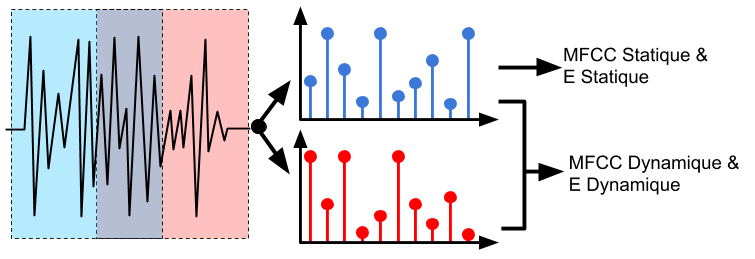
\includegraphics[width=0.75\linewidth]{figures/traitement_signal}}
%   \caption{Traitement du signal audio}
%   \label{fig:traitement_signal}
% \end{figure}
%
%
% \begin{lstlisting}[language=Python, caption={Importer les librairies}, label={code:import}]
% import tensorflow as tf
% \end{lstlisting}


\bibliography{references}

\end{document}
